\subsection{Registrering på PDF}\label{sec:PDF}
Dette afsnit indeholder en gennemgang af grafisk brugergrænseflade, design og implementering af 'Registrering på PDF' viewet i Rambøll Tilsyn.

\subsubsection{Design}
Her under kan sekvensdiagrammerne for registrering på PDF. \\
Det første sekvensdiagram, som ses på figur \ref{fig:LoadPDFSekvensDiagram}, hvordan PDF tegningen bliver loadet ind i applikationen.
\begin{figure}[H] % (alternativt [H])
	\centering
	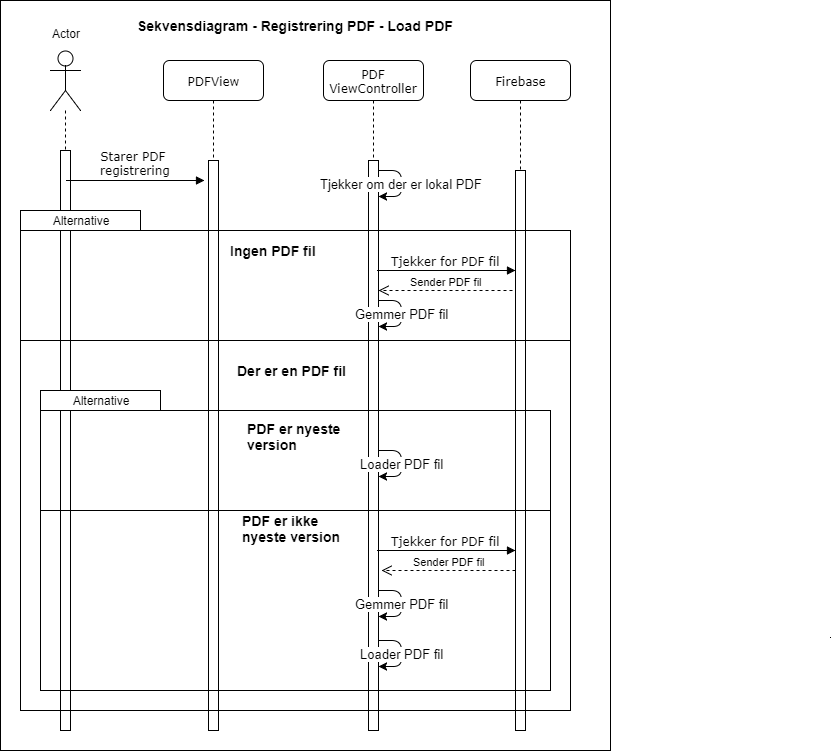
\includegraphics[height=12cm, width=15cm]{../ArkitekturDesign/Design/RegisterPDF/LoadPDFSekvensDiagram}
	\caption{Sekvensdiagram for Registrering på PDF - Loading af PDF, i Rambøll Tilsyn.}
	\label{fig:LoadPDFSekvensDiagram}
\end{figure}

\clearpage

Næste sekvensdiagram, som ses på figur \ref{fig:LoadJSONSekvensDiagram}, viser hvordan JSON filen bliver oprettet. Sekvensen med JSON sker direkte efter at PDF sekvensen er overstået.
\begin{figure}[H] % (alternativt [H])
	\centering
	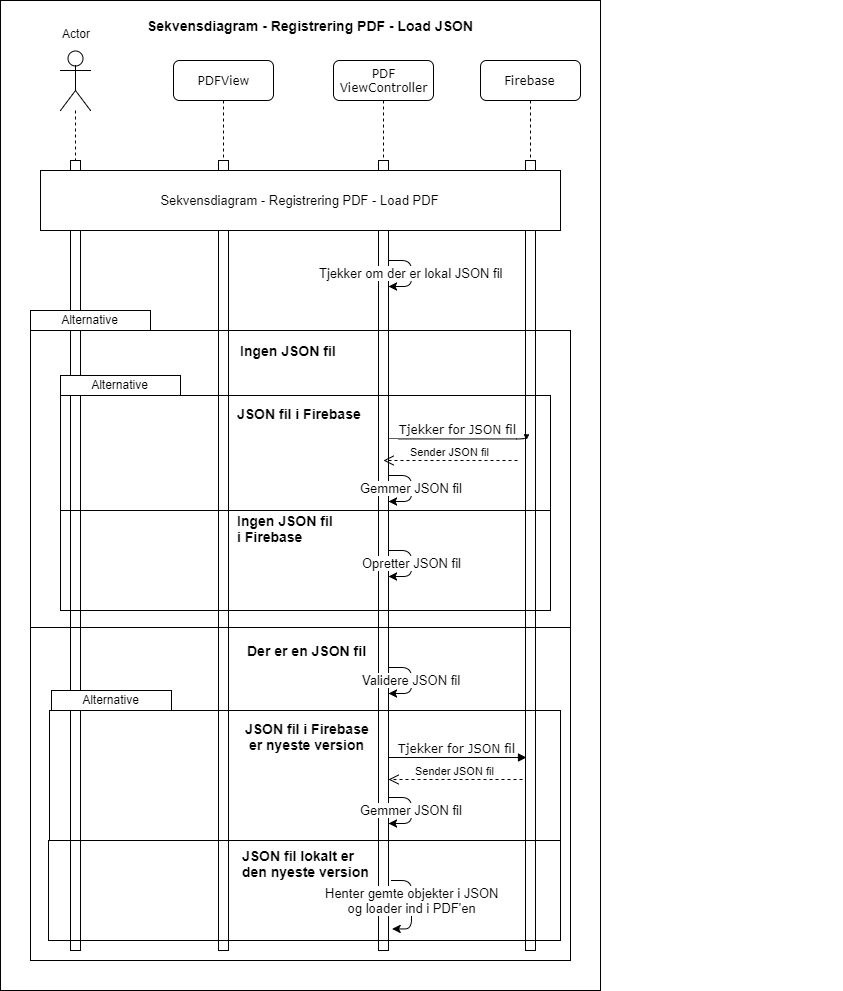
\includegraphics[height=15cm, width=15cm]{../ArkitekturDesign/Design/RegisterPDF/LoadJSONSekvensDiagram}
	\caption{Sekvensdiagram for Registrering på PDF - Loading af JSON, i Rambøll Tilsyn.}
	\label{fig:LoadJSONSekvensDiagram}
\end{figure}

\clearpage

Sidste sekvensdiagram viser hvordan systemet opføre sig, når brugeren interagere med applikationen i forbindelse med oprettelse af objekter på PDF tegningen. Denne sekvens sker i forlængelse af først Loading af PDF og Load JSON. Sekvensdiagrammet for dette kan ses på \ref{fig:RegistrerObjekterSekvensDiagram}.
\begin{figure}[H] % (alternativt [H])
	\centering
	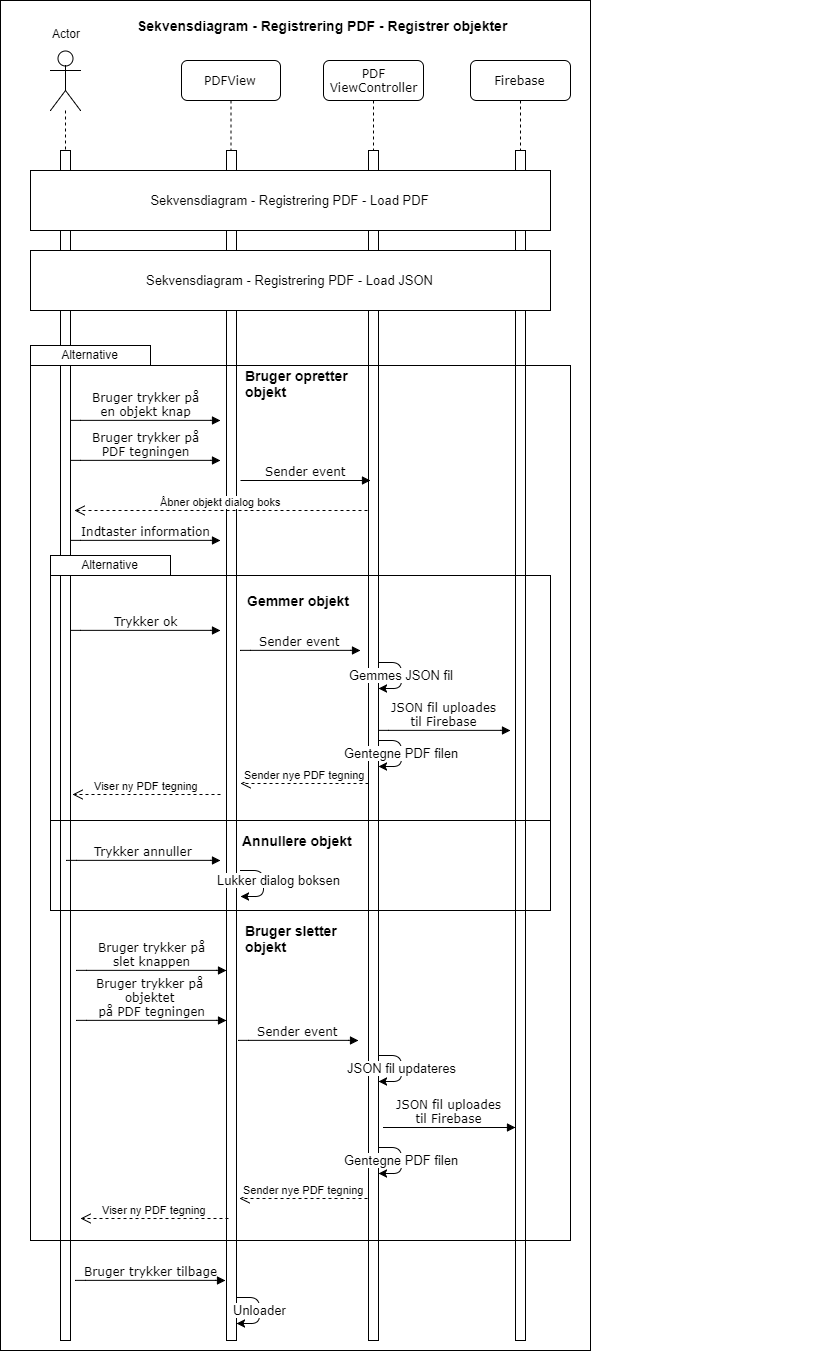
\includegraphics[height=18cm, width=15cm]{../ArkitekturDesign/Design/RegisterPDF/RegistrerObjekterSekvensDiagram}
	\caption{Sekvensdiagram for Registrering på PDF - Registrer på PDF, i Rambøll Tilsyn.}
	\label{fig:RegistrerObjekterSekvensDiagram}
\end{figure}

\clearpage

\subsubsection{Grafisk brugergrænseflade}
RegistrerpåPDFViewet som ses på figur \ref{fig:RegistrerObjekterView} består af to views. Det første view viser den PDF som er valgt til projektet. \\
Under ligger der en andet view som indeholder knapper som brugeren kan interagere med. Der er seks forskellige knapper: \\
Brugeren har mulighed på de første to at enten hoppe en side frem eller en side tilbage. \\
De næste tre knapper er symboler som brugeren kan tegne på PDF'en. \\
Den sidste knap er en liste knap som giver brugeren mulighed for at afslutte sin registrering.
\begin{figure}[H] % (alternativt [H])
	\centering
	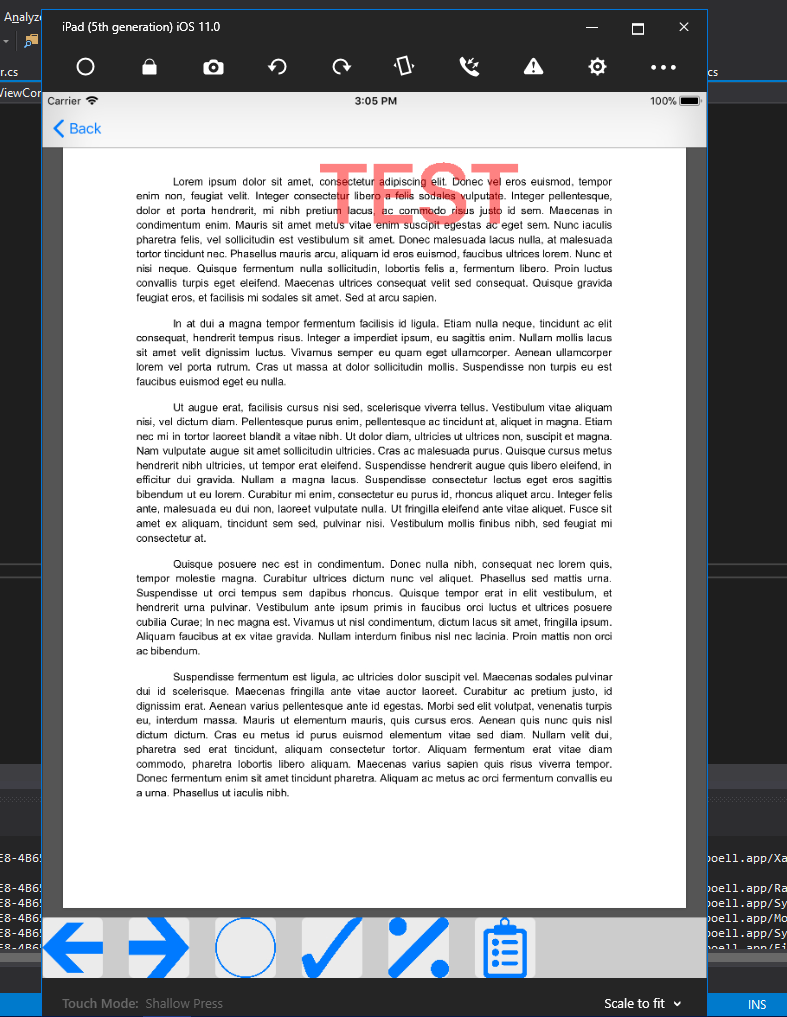
\includegraphics[height=18cm, width=15cm]{../ArkitekturDesign/Design/RegisterPDF/PDF}
	\caption{Registrer på PDF viewet som det er implementeret i Rambøll Tilsyn.}
	\label{fig:RegistrerObjekterView}
\end{figure}

\clearpage

\subsubsection{Implementering}
I dette afsnit vil der blive beskrevet funktionaliteten for de vigtigste funktioner i koden tilhørende 'Registrering på PDF' viewet.

På figur \ref{fig:LoadPDF}, ses funktionen for LoadPDF().
\begin{figure}[H] % (alternativt [H])
	\centering
	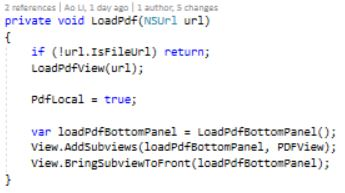
\includegraphics[height=4cm, width=10cm]{../ArkitekturDesign/Design/RegisterPDF/LoadPDF}
	\caption{}
	\label{fig:LoadPDF}
\end{figure}
Efter PDF'en er blevet downloadet fra Firebase, gemmes denne lokalt. \\
Der tjekkes om url'en er en fil url. Er dette en fil url loades PDF'en ind i viewt. \\
Når PDF'en er loadet ind i viewet, oprettes symbol knapperne. \\
Når både PDFViewet og PDFBottomPanel er loadet, loades disse ind i controllerens view.

\clearpage

På figur \ref{fig:LoadPDF}, ses funktionen for LoadBtnPanel().
\begin{figure}[H] % (alternativt [H])
	\centering
	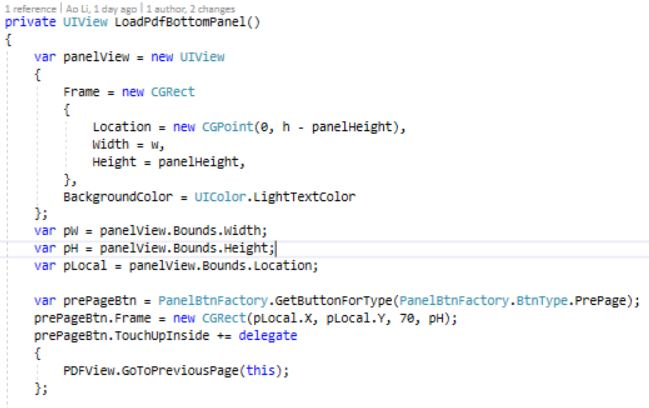
\includegraphics[height=8cm, width=15cm]{../ArkitekturDesign/Design/RegisterPDF/LoadBtnPanel1}
\end{figure}
\begin{figure}[H] % (alternativt [H])
	\centering
	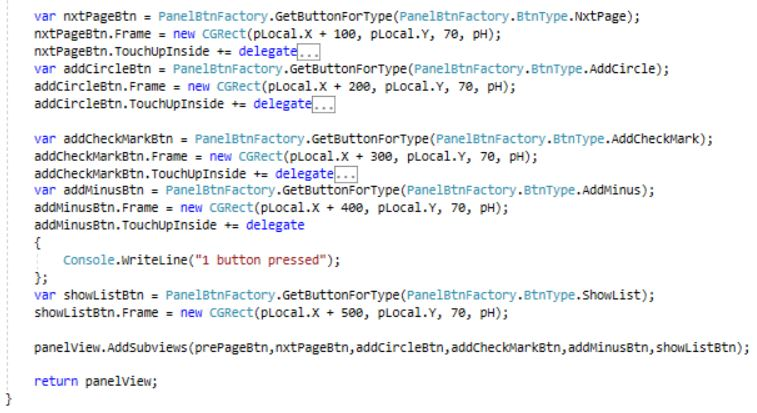
\includegraphics[height=8cm, width=15cm]{../ArkitekturDesign/Design/RegisterPDF/LoadBtnPanel2}
	\caption{}
	\label{fig:LoadBtnPanel2}
\end{figure}
Her oprettes UIView, som indeholder vores knapper, der loades ind fra PanelBottomFactory. \\
PanelBottomFactory er en klasse som står at oprette knapperne. \\
Når knapperne er oprettet definere vi events på de forskellige knapper. \\

\clearpage

På figur \ref{fig:ClassPage}, ses funktionen for ClassPage().
\begin{figure}[H] % (alternativt [H])
	\centering
	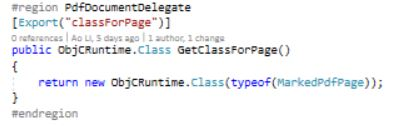
\includegraphics[height=3cm, width=10cm]{../ArkitekturDesign/Design/RegisterPDF/ClassPage}
	\caption{}
	\label{fig:ClassPage}
\end{figure}
Der overrides funktionen ClassForPage, som er en obejktive C funktion, der normalt returnere en standard PDF page, til vores typeof(MarkedPdfPage).

På figur \ref{fig:Draw}, ses funktionen for Draw().
\begin{figure}[H] % (alternativt [H])
	\centering
	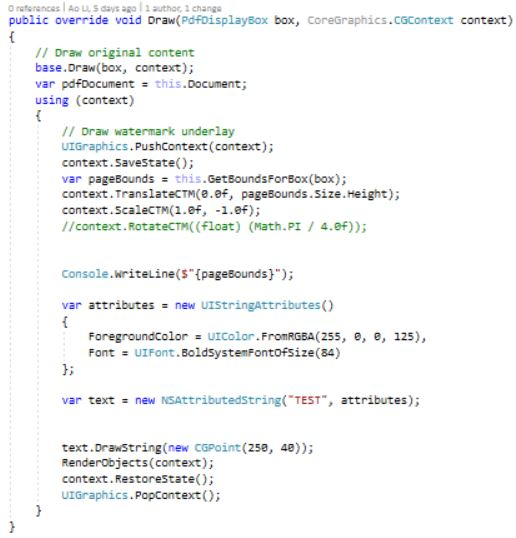
\includegraphics[height=10cm, width=15cm]{../ArkitekturDesign/Design/RegisterPDF/Draw}
	\caption{}
	\label{fig:Draw}
\end{figure}
Når PDF pagen bliver oprettet, kaldes draw og denne er overridet til at tegne på PDF'en med de objekter som bliver hentet fra JSON filen. Disse tegnes ind på PDF'en.

\clearpage

På figur \ref{fig:Enum}, ses funktionen for Render().
\begin{figure}[H] % (alternativt [H])
	\centering
	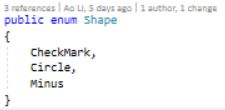
\includegraphics[height=3cm, width=8cm]{../ArkitekturDesign/Design/RegisterPDF/Enum}
	\caption{}
	\label{fig:Enum}
\end{figure}
Definitionen på vores symboler.